%%%%%%%%%%%%%%%%%%%%%%%%%%%%%%%%%%%%%%%%%%
% Engineering problems / LaTeX Template
%		Semester 5
%		Institut d'Optique Graduate School
%%%%%%%%%%%%%%%%%%%%%%%%%%%%%%%%%%%%%%%%%%
%	5N-OptoElec-Bloc1	/ caractérisation statique
%%%%%%%%%%%%%%%%%%%%%%%%%%%%%%%%%%%%%%%%%%
%
% Created by:
%	Julien VILLEMEJANE - 16/jul/2024
% Modified by: Fabienne BERNARD - 30/08/24  Modifs pointées par : %[FaB] 
% Fichier.sty modifié pour changer la police de caractère
%	
%
%%%%%%%%%%%%%%%%%%%%%%%%%%%%%%%%%%%%%%%%%%
% Professional Newsletter Template
% LaTeX Template
% Version 1.0 (09/03/14)
%
% Created by:
% Bob Kerstetter (https://www.tug.org/texshowcase/) and extensively modified by:
% Vel (vel@latextemplates.com)
% 
% This template has been downloaded from:
% http://www.LaTeXTemplates.com
%
% License:
% CC BY-NC-SA 3.0 (http://creativecommons.org/licenses/by-nc-sa/3.0/)
%
%%%%%%%%%%%%%%%%%%%%%%%%%%%%%%%%%%%%%%%%%

\documentclass[a4paper,11pt,titlepage]{article} % The default font size is 10pt; 11pt and 12pt are alternatives

%%%%%%%%%%%%%%%%%%%%%%%%%%%%%%%%%%%%%%%%%%%%%%%%%%%%%%%%%%%%%%%%%%%%%%%%%%%%%%%%%%%%%%%%%%%%%%%%%%%%%%%%%%%%%%%%%%%%%%%%%%%%%%%%%%%%%%%%%%%%%%%%%%%%%%%%%%%%%%%%%%%%%%%%%%%%%%%%%%%%%%%%%%%%%%%%%%%%%%%%%%%%%%%%%%%%%%%%%%%%%%%%%%%%%%%%%%%%%%%%%%%%%%%%%%%%
\usepackage{opto_elec_villemejane}


%%%%%%%%%%%%%%%%%%%%%%%%%%%%%%%%%%%%%%%%%%%%%%%%
%%%%%%%%%%%%%%%%%%%%%%%%%%%%%%%%%%%%%%%%%%%%%%%%
%%%%%%%%%%%%%%%%%%%%%%%%%%%%%%%%%%%%%%%%%%%%%%%%
%%%%%%%%%%%%%%%%%%%%%%%%%%%%%%%%%%%%%%%%%%%%%%%%
\begin{document}



% Page de garde
\begin{titlepage}

\begin{center}
	\begin{minipage}{2.5cm}
	\begin{center}
		
\includegraphics[width=8cm]{images/Logo-LEnsE.png}
	\end{center}
\end{minipage}\hfill
\begin{minipage}{10cm}
	\begin{center}
	\textbf{Institut d'Optique Graduate School }\\[0.1cm]
    \textbf{TP d'Opto-Électronique}


	\end{center}
\end{minipage}\hfill


\vspace{5cm}


{\huge \bfseries \textsc{Opto-Électronique}} \\[0.5cm]
{\large \bfseries Travaux Pratiques} \\[0.2cm]
Semestre 5

\vspace{2cm}
% Title
\rule{\linewidth}{0.3mm} \\[0.4cm]
{ \huge \bfseries\color{violet_iogs} Caractériser un dipôle \\[0.4cm] }
\rule{\linewidth}{0.3mm} \\[1cm]
{\huge Bloc 1}

\vfill

% Bottom of the page
%{\textbf{\large {Année universitaire} 2024-2025}}

\end{center}
\end{titlepage}

\newpage
\strut % empty page
%\cleardoublepage
% Liens vers ressources
\newpage
\pagestyle{empty}

\begin{minipage}[c]{.25\linewidth}
	
\includegraphics[width=5cm]{images/Logo-LEnsE.png}
\end{minipage} \hfill
\begin{minipage}[c]{.4\linewidth}

\begin{center}
\vspace{0.3cm}
{\Large \textsc{Opto-Électronique}}

\medskip

5N-027-SCI \qquad \textbf{\Large TP Bloc 1}

\end{center}
\end{minipage}\hfill

\vspace{0.5cm}

\noindent \rule{\linewidth}{1pt}

{\noindent\Large  \rule[-7pt]{0pt}{30pt}%[FaB]
 \textbf{Caractérisation d'un dipôle}}

\noindent \rule{\linewidth}{1pt}

\bigskip %[FaB]

{\large À l'issue des séances de TP et de TD concernant le bloc 1, les étudiant$\cdot$es seront capables de \textbf{caractériser un dipôle %
électronique} %[FaB]
(linéaire ou non-linéaire) statiquement 
et en \textbf{déduire ses zones de fonctionnement}.}

\medskip

\textit{Les sujets de TD ne sont pas inclus dans ce document.}

\medskip

\textit{Ce sujet est disponible au format électronique sur le site du LEnsE - https://lense.institutoptique.fr/ dans la rubrique Année / Première Année / Opto-Electronique S5 / Bloc 1.}

\noindent \rule{\linewidth}{1pt}

\medskip

Pour cela, ils$\cdot$elles %[FaB]devront être
seront capables de~:

\begin{itemize}
	\item Lister %
	les grandeurs et les %[FaB]
	paramètres d'intérêt %importants 
	du composant à partir d'une documentation technique fournie
	\item Choisir les paramètres des instruments de mesures et des composants de protection
	\item Tracer la caractéristique statique à l'aide :
	\begin{itemize}
		\item d'un multimètre
		\item d'un oscilloscope en mode XY
	\end{itemize}
	\item Décrire le fonctionnement d'un montage à diodes
\end{itemize}


\noindent \rule{\linewidth}{1pt}

\medskip

\textbf{\large Liste des missions}

\begin{description}
	\item[Mission 1.1] \hyperref[mission11]{Tracer la caractéristique $i=f(u)$ d'une photodiode}
	\item[Mission 1.2] \hyperref[mission12]{Mesurer le courant généré par une photodiode en mode capteur}
	\item[Mission 1.3] \hyperref[mission13]{Tracer la caractéristique $i = f(u)$ d'un dipôle de manière automatisée}
	\item[Mission 1.4] \hyperref[mission14]{Tracer la caractéristique $i = f(u)$ d'une LED}
\end{description}

\noindent \rule{\linewidth}{1pt}

\medskip

\textbf{\large Liste des autres ressources}
\begin{itemize}
	\item \hyperref[ressource:CaracStat]{Caractériser un dipôle}
	\item \hyperref[doc:phdSFH206K]{Doc : SFH206K (photodiode)}
	\item \hyperref[doc:ledRouge]{Doc : LED rouge}
	\item \hyperref[fiche:Led]{Fiche : Diode / LED / Photodiode}
	\item \hyperref[fiche:Photodetect]{Fiche : Photodétection}
\end{itemize}

\medskip

Un \textbf{feuillet annexe}, présentant succinctement l'\textbf{ensemble des instruments}, est disponible sur chacune des paillasses.


\newpage
\strut % empty page
% Missions
%[FaB]\newpage
%\pagestyle{empty}

\begin{minipage}[c]{.25\linewidth}
	
\includegraphics[width=4cm]{images/Logo-LEnsE.png}
\end{minipage} \hfill
\begin{minipage}[c]{.4\linewidth}

\begin{center}
\vspace{0.3cm}
{\Large \textsc{Opto-Électronique}}

\medskip

5N-027-SCI \qquad \textbf{\Large TP Bloc 1}

\end{center}
\end{minipage}\hfill

\vspace{0.5cm}

\noindent \rule{\linewidth}{1pt}

{\noindent\Large \rule[-7pt]{0pt}{30pt} \textbf{Mission 1.1} / Tracer la caractéristique $i = f(u)$ d'une photodiode} 

\noindent \rule{\linewidth}{1pt}

\vspace{-0.5cm}

\begin{center}

Durée conseillée : 60 min / Séance 1

\end{center}

%%%%%%%%%%%%%%%%%%%%%%%%%%%%%%%%%%
\section{Objectif de la mission}
\label{mission11}

On se propose de \textbf{caractériser une photodiode}, c'est à dire de \textbf{tracer expérimentalement la loi mathématique} qui lie le courant traversant le dipôle et la différence de potentiel à ses bornes.


%%%%%%%%%%%%%%%%%%%%%%%%%%%%%%%%%%
%%%%%%%%%%%%%%%%%%%%%%%%%%%%%%%%%%
%%%%%%%%%%%%%%%%%%%%%%%%%%%%%%%%%%
\section{Ressources}

Vous pouvez utiliser les fiches résumées suivantes : 

\begin{itemize}
	\item \hyperref[fiche:Led]{Fiche : Diode / LED / Photodiode}
	\item \hyperref[fiche:Photodetect]{Fiche : Photodétection}
\end{itemize}


\subsection{Photodiode \texttt{SFH206K}}

On utilisera une photodiode de type \textbf{\texttt{SFH206K}} (une partie de la \hyperref[doc:phdSFH206K]{documentation} est fournie en annexe).

\Quest Rechercher et relever dans la documentation technique du constructeur de la photodiode \texttt{SFH206K} les valeurs intéressantes pour la mise en \oe{}uvre pratique (électrique et optique) d'un tel composant.


\subsection{Méthode conventionnelle}

Vous utiliserez une méthode classique de l'instrumentation pour relever les points de la courbe $i = f(u)$. Vous pourrez vous inspirer de la partie \textbf{Caractéristique manuelle} du tutoriel \hyperref[ressource:CaracStat]{Caractériser un dipôle}.

\subsection{Choix des appareils et des composants}

Dans le schéma proposé dans le tutoriel \textbf{Caractéristique manuelle} du tutoriel \hyperref[ressource:CaracStat]{Caractériser un dipôle}, une résistance $R_P$ est proposée comme protection en courant.

\Quest Comment choisir cette résistance et comment régler les différents appareils de mesure?

\Manip Relever la caractéristique $i=f(u)$ de cette photodiode, lorsqu'elle est plongée dans l'obscurité, pour des tensions $u$ positives ET négatives.


%%%%%%%%%%%%%%%%%%%%%%%%%%%%%%%%%%
\section{Livrables}


Une \textbf{fiche de manipulation} en ligne (partagée dans le cahier de laboratoire) rappelant :

\begin{itemize}
	\item les protocoles de mesure et de réglage (schémas de mesure, de câblage)
	\item les tableaux de mesures et les courbes obtenues
\end{itemize}

Une \textbf{analyse} du résultat obtenu, en particulier sur les valeurs de courant obtenues pour une tension négative en présence ou non de photons.

%%%%%%%%%%%%%%%%%%%%%%%%%%%%%%%%%%%%%%%%%%%%%%%%%%%%%%%%%%%%%%%%%%%%%%%%%%%%%%%%%%%%%
\newpage
%\pagestyle{empty}

\begin{minipage}[c]{.25\linewidth}
	
\includegraphics[width=4cm]{images/Logo-LEnsE.png}
\end{minipage} \hfill
\begin{minipage}[c]{.4\linewidth}

\begin{center}
\vspace{0.3cm}
{\Large \textsc{Opto-Électronique}}

\medskip

5N-027-SCI \qquad \textbf{\Large TP Bloc 1}

\end{center}
\end{minipage}\hfill

\vspace{0.5cm}

\noindent \rule{\linewidth}{1pt}

{\noindent\Large \rule[-7pt]{0pt}{30pt} \textbf{Mission 1.1} / Tracer la caractéristique $i = f(u)$ d'une photodiode} 

\noindent \rule{\linewidth}{1pt}

\vspace{-0.5cm}

\begin{center}

Durée conseillée : 60 min / Séance 1

\end{center}

%%%%%%%%%%%%%%%%%%%%%%%%%%%%%%%%%%
\section{Objectif de la mission}
\label{mission11}

On se propose de \textbf{caractériser une photodiode}, c'est à dire de \textbf{tracer expérimentalement la loi mathématique} qui lie le courant traversant le dipôle et la différence de potentiel à ses bornes.


%%%%%%%%%%%%%%%%%%%%%%%%%%%%%%%%%%
%%%%%%%%%%%%%%%%%%%%%%%%%%%%%%%%%%
%%%%%%%%%%%%%%%%%%%%%%%%%%%%%%%%%%
\section{Ressources}

Vous pouvez utiliser les fiches résumées suivantes : 

\begin{itemize}
	\item \hyperref[fiche:Led]{Fiche : Diode / LED / Photodiode}
	\item \hyperref[fiche:Photodetect]{Fiche : Photodétection}
\end{itemize}


\subsection{Photodiode \texttt{SFH206K}}

On utilisera une photodiode de type \textbf{\texttt{SFH206K}} (une partie de la \hyperref[doc:phdSFH206K]{documentation} est fournie en annexe).

\Quest Rechercher et relever dans la documentation technique du constructeur de la photodiode \texttt{SFH206K} les valeurs intéressantes pour la mise en \oe{}uvre pratique (électrique et optique) d'un tel composant.


\subsection{Méthode conventionnelle}

Vous utiliserez une méthode classique de l'instrumentation pour relever les points de la courbe $i = f(u)$. Vous pourrez vous inspirer de la partie \textbf{Caractéristique manuelle} du tutoriel \hyperref[ressource:CaracStat]{Caractériser un dipôle}.

\subsection{Choix des appareils et des composants}

Dans le schéma proposé dans le tutoriel \textbf{Caractéristique manuelle} du tutoriel \hyperref[ressource:CaracStat]{Caractériser un dipôle}, une résistance $R_P$ est proposée comme protection en courant.

\Quest Comment choisir cette résistance et comment régler les différents appareils de mesure?

\Manip Relever la caractéristique $i=f(u)$ de cette photodiode, lorsqu'elle est plongée dans l'obscurité, pour des tensions $u$ positives ET négatives.


%%%%%%%%%%%%%%%%%%%%%%%%%%%%%%%%%%
\section{Livrables}


Une \textbf{fiche de manipulation} en ligne (partagée dans le cahier de laboratoire) rappelant :

\begin{itemize}
	\item les protocoles de mesure et de réglage (schémas de mesure, de câblage)
	\item les tableaux de mesures et les courbes obtenues
\end{itemize}

Une \textbf{analyse} du résultat obtenu, en particulier sur les valeurs de courant obtenues pour une tension négative en présence ou non de photons.

%%%%%%%%%%%%%%%%%%%%%%%%%%%%%%%%%%%%%%%%%%%%%%%%%%%%%%%%%%%%%%%%%%%%%%%%%%%%%%%%%%%%%

%[FaB]\newpage
\pagestyle{empty}

\begin{minipage}[c]{.25\linewidth}
	
\includegraphics[width=4cm]{images/Logo-LEnsE.png}
\end{minipage} \hfill
\begin{minipage}[c]{.4\linewidth}

\begin{center}
\vspace{0.3cm}
{\Large \textsc{Opto-Électronique}}

\medskip

5N-027-SCI \qquad \textbf{\Large TP Bloc 1}

\end{center}
\end{minipage}\hfill

\vspace{0.5cm}

\noindent \rule{\linewidth}{1pt}

{\noindent\Large  \rule[-7pt]{0pt}{30pt}  \textbf{Mission 1.2} / Mesurer le courant généré par une photodiode en mode capteur} 

\noindent \rule{\linewidth}{1pt}

\vspace{-0.5cm}

\begin{center}

Durée conseillée : 30 min / Séance 1

\end{center}

%%%%%%%%%%%%%%%%%%%%%%%%%%%%%%%%%%
\section{Objectif de la mission}
\label{mission12}

On souhaite \textbf{mesurer le courant généré par une photodiode} (dans le domaine du visible) à l'aide d'un ampèremètre pour différentes valeurs d'éclairement.


%%%%%%%%%%%%%%%%%%%%%%%%%%%%%%%%%%
%%%%%%%%%%%%%%%%%%%%%%%%%%%%%%%%%%
%%%%%%%%%%%%%%%%%%%%%%%%%%%%%%%%%%
\section{Ressources}

Vous pouvez utiliser les fiches résumées suivantes : 

\begin{itemize}
	\item \hyperref[fiche:Led]{Fiche : Diode / LED / Photodiode}
	\item \hyperref[fiche:Photodetect]{Fiche : Photodétection}
\end{itemize}

\subsection{Utilisation d'un luxmètre}

Afin d'avoir une donnée de comparaison d'éclairement ambiant de la salle de travaux pratiques, un luxmètre est mis à votre disposition.

Vous pourrez ainsi comparer certaines données du constructeur avec vos résultats...


\Manip A l'aide d'un luxmètre, relever des valeurs d'éclairement :
\begin{itemize}
	\item dans l'obscurité,
	\item de la paillasse éclairée avec l'éclairage ambiant,
	\item de la paillasse éclairée avec une source supplémentaire (lampe de bureau ou lampe du téléphone portable).
\end{itemize}

\Manip Relever les valeurs du courant $i$ obtenu en sortie de la photodiode dans les trois conditions d'éclairage précédentes, pour une tension directe de l'ordre de $1\operatorname{V}$ et pour une tension inverse de $5\operatorname{V}$ (tension mesurée dans l'obscurité).

\Quest Dans quel cas est-il plus intéressant d'utiliser cette photodiode comme capteur de photons ?


%%%%%%%%%%%%%%%%%%%%%%%%%%%%%%%%%%
\section{Livrables}


Une \textbf{fiche de manipulation} en ligne (partagée dans le cahier de laboratoire) rappelant :

\begin{itemize}
	\item les protocoles de mesure et de réglage (schémas de mesure, de câblage)
	\item les tableaux de mesures obtenues
\end{itemize}

Une \textbf{analyse} du résultat obtenu et une comparaison entre les valeurs expérimentale et théorique obtenues pour le courant en présence du flux lumineux ambiant.

%%%%%%%%%%%%%%%%%%%%%%%%%%%%%%%%%%%%%%%%%%%%%%%%%%%%%%%%%%%%%%%%%%%%%%%%%%%%%%%%%%%%%

\newpage
\pagestyle{empty}

\begin{minipage}[c]{.25\linewidth}
	
\includegraphics[width=4cm]{images/Logo-LEnsE.png}
\end{minipage} \hfill
\begin{minipage}[c]{.4\linewidth}

\begin{center}
\vspace{0.3cm}
{\Large \textsc{Opto-Électronique}}

\medskip

5N-027-SCI \qquad \textbf{\Large TP Bloc 1}

\end{center}
\end{minipage}\hfill

\vspace{0.5cm}

\noindent \rule{\linewidth}{1pt}

{\noindent\Large  \rule[-7pt]{0pt}{30pt}  \textbf{Mission 1.2} / Mesurer le courant généré par une photodiode en mode capteur} 

\noindent \rule{\linewidth}{1pt}

\vspace{-0.5cm}

\begin{center}

Durée conseillée : 30 min / Séance 1

\end{center}

%%%%%%%%%%%%%%%%%%%%%%%%%%%%%%%%%%
\section{Objectif de la mission}
\label{mission12}

On souhaite \textbf{mesurer le courant généré par une photodiode} (dans le domaine du visible) à l'aide d'un ampèremètre pour différentes valeurs d'éclairement.


%%%%%%%%%%%%%%%%%%%%%%%%%%%%%%%%%%
%%%%%%%%%%%%%%%%%%%%%%%%%%%%%%%%%%
%%%%%%%%%%%%%%%%%%%%%%%%%%%%%%%%%%
\section{Ressources}

Vous pouvez utiliser les fiches résumées suivantes : 

\begin{itemize}
	\item \hyperref[fiche:Led]{Fiche : Diode / LED / Photodiode}
	\item \hyperref[fiche:Photodetect]{Fiche : Photodétection}
\end{itemize}

\subsection{Utilisation d'un luxmètre}

Afin d'avoir une donnée de comparaison d'éclairement ambiant de la salle de travaux pratiques, un luxmètre est mis à votre disposition.

Vous pourrez ainsi comparer certaines données du constructeur avec vos résultats...


\Manip A l'aide d'un luxmètre, relever des valeurs d'éclairement :
\begin{itemize}
	\item dans l'obscurité,
	\item de la paillasse éclairée avec l'éclairage ambiant,
	\item de la paillasse éclairée avec une source supplémentaire (lampe de bureau ou lampe du téléphone portable).
\end{itemize}

\Manip Relever les valeurs du courant $i$ obtenu en sortie de la photodiode dans les trois conditions d'éclairage précédentes, pour une tension directe de l'ordre de $1\operatorname{V}$ et pour une tension inverse de $5\operatorname{V}$ (tension mesurée dans l'obscurité).

\Quest Dans quel cas est-il plus intéressant d'utiliser cette photodiode comme capteur de photons ?


%%%%%%%%%%%%%%%%%%%%%%%%%%%%%%%%%%
\section{Livrables}


Une \textbf{fiche de manipulation} en ligne (partagée dans le cahier de laboratoire) rappelant :

\begin{itemize}
	\item les protocoles de mesure et de réglage (schémas de mesure, de câblage)
	\item les tableaux de mesures obtenues
\end{itemize}

Une \textbf{analyse} du résultat obtenu et une comparaison entre les valeurs expérimentale et théorique obtenues pour le courant en présence du flux lumineux ambiant.

%%%%%%%%%%%%%%%%%%%%%%%%%%%%%%%%%%%%%%%%%%%%%%%%%%%%%%%%%%%%%%%%%%%%%%%%%%%%%%%%%%%%%

%[FaB]\newpage
\pagestyle{empty}

\begin{minipage}[c]{.25\linewidth}
	
\includegraphics[width=4cm]{images/Logo-LEnsE.png}
\end{minipage} \hfill
\begin{minipage}[c]{.4\linewidth}

\begin{center}
\vspace{0.3cm}
{\Large \textsc{Opto-Électronique}}

\medskip

5N-027-SCI \qquad \textbf{\Large TP Bloc 1}

\end{center}
\end{minipage}\hfill

\vspace{0.5cm}

\noindent \rule{\linewidth}{1pt}

{\noindent\Large \rule[-7pt]{0pt}{30pt} \textbf{Mission 1.3} / Tracer la caractéristique $i = f(u)$ d'un dipôle de manière automatisée} 

\noindent \rule{\linewidth}{1pt}

\vspace{-0.5cm}

\begin{center}

Durée conseillée : 60 min / Séance 2

\end{center}

%%%%%%%%%%%%%%%%%%%%%%%%%%%%%%%%%%
\section{Objectif de la mission}
\label{mission13}

On souhaite \textbf{caractériser une photodiode} (dans le domaine du visible), c'est à dire \textbf{tracer expérimentalement la loi mathématique} qui lie le courant traversant le dipôle et la différence de potentiel à ses bornes de manière plus automatisée que lors de la mission 1.1.

On souhaite voir également l'évolution de cette caractéristique en fonction de l'éclairement de la photodiode.


%%%%%%%%%%%%%%%%%%%%%%%%%%%%%%%%%%
%%%%%%%%%%%%%%%%%%%%%%%%%%%%%%%%%%
%%%%%%%%%%%%%%%%%%%%%%%%%%%%%%%%%%
\section{Ressources}

Vous pouvez utiliser les fiches résumées suivantes : 

\begin{itemize}
	\item \hyperref[fiche:Led]{Fiche : Diode / LED / Photodiode}
	\item \hyperref[fiche:Photodetect]{Fiche : Photodétection}
\end{itemize}


\subsection{Méthode automatisée}

Vous utiliserez cette fois-ci une méthode plus rapide pour relever une allure de la courbe $i = f(u)$. Vous pourrez vous inspirer de la partie \textbf{Caractéristique automatique} du tutoriel \hyperref[ressource:CaracStat]{Caractériser un dipôle}.

\Manip Relever la caractéristique statique de la photodiode dans les deux cas suivants:

\begin{itemize}
	\item dans l'obscurité
	\item en présence d'un flux lumineux (fourni par une source externe)
\end{itemize}

\Manip Mesurer, à l'aide d'un luxmètre, le flux lumineux émis par la source externe utilisée.



%%%%%%%%%%%%%%%%%%%%%%%%%%%%%%%%%%
\section{Livrables}


Une \textbf{fiche de manipulation} en ligne (partagée dans le cahier de laboratoire) rappelant :

\begin{itemize}
	\item les protocoles de mesure et de réglage (schémas de mesure, de câblage)
	\item les tableaux de mesures et les courbes obtenues, %
	copies d'écran d'oscilloscope en particulier %[FaB]
\end{itemize}

Une \textbf{analyse} du résultat obtenu et des zones d'utilisation possible d'une photodiode. On s'intéressera en particulier à la zone qui permet de mesurer un flux lumineux.

%%%%%%%%%%%%%%%%%%%%%%%%%%%%%%%%%%%%%%%%%%%%%%%%%%%%%%%%%%%%%%%%%%%%%%%%%%%%%%%%%%%%%

\newpage
\pagestyle{empty}

\begin{minipage}[c]{.25\linewidth}
	
\includegraphics[width=4cm]{images/Logo-LEnsE.png}
\end{minipage} \hfill
\begin{minipage}[c]{.4\linewidth}

\begin{center}
\vspace{0.3cm}
{\Large \textsc{Opto-Électronique}}

\medskip

5N-027-SCI \qquad \textbf{\Large TP Bloc 1}

\end{center}
\end{minipage}\hfill

\vspace{0.5cm}

\noindent \rule{\linewidth}{1pt}

{\noindent\Large \rule[-7pt]{0pt}{30pt} \textbf{Mission 1.3} / Tracer la caractéristique $i = f(u)$ d'un dipôle de manière automatisée} 

\noindent \rule{\linewidth}{1pt}

\vspace{-0.5cm}

\begin{center}

Durée conseillée : 60 min / Séance 2

\end{center}

%%%%%%%%%%%%%%%%%%%%%%%%%%%%%%%%%%
\section{Objectif de la mission}
\label{mission13}

On souhaite \textbf{caractériser une photodiode} (dans le domaine du visible), c'est à dire \textbf{tracer expérimentalement la loi mathématique} qui lie le courant traversant le dipôle et la différence de potentiel à ses bornes de manière plus automatisée que lors de la mission 1.1.

On souhaite voir également l'évolution de cette caractéristique en fonction de l'éclairement de la photodiode.


%%%%%%%%%%%%%%%%%%%%%%%%%%%%%%%%%%
%%%%%%%%%%%%%%%%%%%%%%%%%%%%%%%%%%
%%%%%%%%%%%%%%%%%%%%%%%%%%%%%%%%%%
\section{Ressources}

Vous pouvez utiliser les fiches résumées suivantes : 

\begin{itemize}
	\item \hyperref[fiche:Led]{Fiche : Diode / LED / Photodiode}
	\item \hyperref[fiche:Photodetect]{Fiche : Photodétection}
\end{itemize}


\subsection{Méthode automatisée}

Vous utiliserez cette fois-ci une méthode plus rapide pour relever une allure de la courbe $i = f(u)$. Vous pourrez vous inspirer de la partie \textbf{Caractéristique automatique} du tutoriel \hyperref[ressource:CaracStat]{Caractériser un dipôle}.

\Manip Relever la caractéristique statique de la photodiode dans les deux cas suivants:

\begin{itemize}
	\item dans l'obscurité
	\item en présence d'un flux lumineux (fourni par une source externe)
\end{itemize}

\Manip Mesurer, à l'aide d'un luxmètre, le flux lumineux émis par la source externe utilisée.



%%%%%%%%%%%%%%%%%%%%%%%%%%%%%%%%%%
\section{Livrables}


Une \textbf{fiche de manipulation} en ligne (partagée dans le cahier de laboratoire) rappelant :

\begin{itemize}
	\item les protocoles de mesure et de réglage (schémas de mesure, de câblage)
	\item les tableaux de mesures et les courbes obtenues, %
	copies d'écran d'oscilloscope en particulier %[FaB]
\end{itemize}

Une \textbf{analyse} du résultat obtenu et des zones d'utilisation possible d'une photodiode. On s'intéressera en particulier à la zone qui permet de mesurer un flux lumineux.

%%%%%%%%%%%%%%%%%%%%%%%%%%%%%%%%%%%%%%%%%%%%%%%%%%%%%%%%%%%%%%%%%%%%%%%%%%%%%%%%%%%%%

%[FaB]
\newpage
\pagestyle{empty}

\begin{minipage}[c]{.25\linewidth}
	
\includegraphics[width=4cm]{images/Logo-LEnsE.png}
\end{minipage} \hfill
\begin{minipage}[c]{.4\linewidth}

\begin{center}
\vspace{0.3cm}
{\Large \textsc{Opto-Électronique}}

\medskip

5N-027-SCI \qquad \textbf{\Large TP Bloc 1}

\end{center}
\end{minipage}\hfill

\vspace{0.5cm}

\noindent \rule{\linewidth}{1pt}

{\noindent\Large \rule[-7pt]{0pt}{30pt}  \textbf{Mission 1.4} / Tracer la caractéristique $i = f(u)$ d'une LED} 

\noindent \rule{\linewidth}{1pt}

\vspace{-0.5cm}

\begin{center}

Durée conseillée : 30 min / Séance 3 ou 4

\end{center}

%%%%%%%%%%%%%%%%%%%%%%%%%%%%%%%%%%
\section{Objectif de la mission}
\label{mission14}

On souhaite \textbf{caractériser une LED rouge}, c'est à dire \textbf{tracer expérimentalement la loi mathématique} qui lie le courant traversant le dipôle et la différence de potentiel à ses bornes, afin de déterminer un point de fonctionnement idéal pour transmettre un signal sinusoïdal.


%%%%%%%%%%%%%%%%%%%%%%%%%%%%%%%%%%
%%%%%%%%%%%%%%%%%%%%%%%%%%%%%%%%%%
%%%%%%%%%%%%%%%%%%%%%%%%%%%%%%%%%%
\section{Ressources}

Vous pouvez utiliser la fiche résumée suivante : 

\begin{itemize}
	\item \hyperref[fiche:Led]{Fiche : Diode / LED / Photodiode}
\end{itemize}

\subsection{LED Rouge}

On utilisera une LED rouge de type \texttt{Kingbrigth L-1503ID} (une partie de la \hyperref[doc:ledRouge]{documentation} est fournie en annexe).

\Quest Rechercher et relever dans la documentation technique du constructeur de la LED les valeurs intéressantes pour la mise en oeuvre pratique (électrique et optique) d'un tel composant.

\subsection{Méthode automatisée}

Vous utiliserez cette fois-ci une méthode plus rapide pour relever une allure de la courbe $i = f(u)$. Vous pourrez vous inspirer de la partie \textbf{Caractéristique automatique} du tutoriel \hyperref[ressource:CaracStat]{Caractériser un dipôle}.

\Quest Comment choisir la résistance de protection de la LED ? Comment régler les différents appareils de mesure pour éviter de dégrader la LED ?

\Manip Relever la caractéristique statique de la LED.


%%%%%%%%%%%%%%%%%%%%%%%%%%%%%%%%%%
\section{Livrables}


Une \textbf{fiche de manipulation} en ligne (partagée dans le cahier de laboratoire) rappelant :

\begin{itemize}
	\item les protocoles de mesure et de réglage (schémas de mesure, de câblage)
	\item les tableaux de mesures et les courbes obtenues
\end{itemize}

Une \textbf{analyse} du résultat obtenu.

Quelques lignes expliquant :

\begin{itemize}
	\item dans quelle zone la LED peut-être utilisée pour moduler la lumière émise,
	\item les précautions à prendre pour obtenir une modulation sinusoïdale du flux lumineux.
\end{itemize}

%%%%%%%%%%%%%%%%%%%%%%%%%%%%%%%%%%%%%%%%%%%%%%%%%%%%%%%%%%%%%%%%%%%%%%%%%%%%%%%%%%%%%


\newpage
\pagestyle{empty}

\begin{minipage}[c]{.25\linewidth}
	
\includegraphics[width=4cm]{images/Logo-LEnsE.png}
\end{minipage} \hfill
\begin{minipage}[c]{.4\linewidth}

\begin{center}
\vspace{0.3cm}
{\Large \textsc{Opto-Électronique}}

\medskip

5N-027-SCI \qquad \textbf{\Large TP Bloc 1}

\end{center}
\end{minipage}\hfill

\vspace{0.5cm}

\noindent \rule{\linewidth}{1pt}

{\noindent\Large \rule[-7pt]{0pt}{30pt}  \textbf{Mission 1.4} / Tracer la caractéristique $i = f(u)$ d'une LED} 

\noindent \rule{\linewidth}{1pt}

\vspace{-0.5cm}

\begin{center}

Durée conseillée : 30 min / Séance 3 ou 4

\end{center}

%%%%%%%%%%%%%%%%%%%%%%%%%%%%%%%%%%
\section{Objectif de la mission}
\label{mission14}

On souhaite \textbf{caractériser une LED rouge}, c'est à dire \textbf{tracer expérimentalement la loi mathématique} qui lie le courant traversant le dipôle et la différence de potentiel à ses bornes, afin de déterminer un point de fonctionnement idéal pour transmettre un signal sinusoïdal.


%%%%%%%%%%%%%%%%%%%%%%%%%%%%%%%%%%
%%%%%%%%%%%%%%%%%%%%%%%%%%%%%%%%%%
%%%%%%%%%%%%%%%%%%%%%%%%%%%%%%%%%%
\section{Ressources}

Vous pouvez utiliser la fiche résumée suivante : 

\begin{itemize}
	\item \hyperref[fiche:Led]{Fiche : Diode / LED / Photodiode}
\end{itemize}

\subsection{LED Rouge}

On utilisera une LED rouge de type \texttt{Kingbrigth L-1503ID} (une partie de la \hyperref[doc:ledRouge]{documentation} est fournie en annexe).

\Quest Rechercher et relever dans la documentation technique du constructeur de la LED les valeurs intéressantes pour la mise en oeuvre pratique (électrique et optique) d'un tel composant.

\subsection{Méthode automatisée}

Vous utiliserez cette fois-ci une méthode plus rapide pour relever une allure de la courbe $i = f(u)$. Vous pourrez vous inspirer de la partie \textbf{Caractéristique automatique} du tutoriel \hyperref[ressource:CaracStat]{Caractériser un dipôle}.

\Quest Comment choisir la résistance de protection de la LED ? Comment régler les différents appareils de mesure pour éviter de dégrader la LED ?

\Manip Relever la caractéristique statique de la LED.


%%%%%%%%%%%%%%%%%%%%%%%%%%%%%%%%%%
\section{Livrables}


Une \textbf{fiche de manipulation} en ligne (partagée dans le cahier de laboratoire) rappelant :

\begin{itemize}
	\item les protocoles de mesure et de réglage (schémas de mesure, de câblage)
	\item les tableaux de mesures et les courbes obtenues
\end{itemize}

Une \textbf{analyse} du résultat obtenu.

Quelques lignes expliquant :

\begin{itemize}
	\item dans quelle zone la LED peut-être utilisée pour moduler la lumière émise,
	\item les précautions à prendre pour obtenir une modulation sinusoïdale du flux lumineux.
\end{itemize}

%%%%%%%%%%%%%%%%%%%%%%%%%%%%%%%%%%%%%%%%%%%%%%%%%%%%%%%%%%%%%%%%%%%%%%%%%%%%%%%%%%%%%



\newpage
% Ressources
\begin{center}
	\begin{minipage}{2.5cm}
	\begin{center}
		
\includegraphics[width=5cm]{images/Logo-LEnsE.png}
	\end{center}
\end{minipage}\hfill
\begin{minipage}{10cm}
	\begin{center}
	\textbf{Institut d'Optique Graduate School }\\[0.1cm]
    \textbf{TP d'Opto-Électronique}


	\end{center}
\end{minipage}\hfill


\vspace{2cm}


{\Large \bfseries \textsc{Opto-Électronique}} \\[0.5cm]
{\large \bfseries Travaux Pratiques} \\[0.2cm]
Semestre 5

\vspace{1cm}

% Title
\rule{\linewidth}{0.4mm} \\[0.4cm]
{ \Large \bfseries\color{violet_iogs} Ressources \\[0.4cm] }
\rule{\linewidth}{0.4mm} \\[1cm]
{\large Bloc 1}

\end{center}

\vspace{3cm}

\textbf{\large Liste des ressources}
\begin{itemize}
	\item \hyperref[ressource:CaracStat]{Caractériser un dipôle}
	\begin{itemize}
		\item \textit{Caractéristique Manuelle}
		\item \textit{Caractéristique Automatisée}
	\end{itemize}
	\item \hyperref[doc:phdSFH206K]{Doc : SFH206K (photodiode)}
	\item \hyperref[doc:ledRouge]{Doc : LED rouge}
	\item \hyperref[fiche:Led]{Fiche : Diode / LED / Photodiode}
	\item \hyperref[fiche:Photodetect]{Fiche : Photodétection}
\end{itemize}

\vfill

\newpage
\strut % empty page

\newpage
\pagestyle{empty}

\begin{minipage}[c]{.25\linewidth}
	
\includegraphics[width=4cm]{images/Logo-LEnsE.png}
\end{minipage} \hfill
\begin{minipage}[c]{.4\linewidth}

\begin{center}
\vspace{0.3cm}
{\Large \textsc{Opto-Électronique}}

\medskip

\textbf{\Large Ressources}

\end{center}
\end{minipage}\hfill

\vspace{0.5cm}

\noindent \rule{\linewidth}{1pt}
\section{Caractéristique statique d'un dipôle}
\label{ressource:CaracStat}


%%%%%%%%%%%%%%%%%%%%%%%%%%%%%%%%%%%%%%%%%%%%%%%%%%%%%%%%%%%%%%%%%%%%%%%%%%%%%%%%
%%%%%

En électronique, la caractéristique statique d'un dipôle correspond à la relation mathématique $i=f(u)$ qu'il existe entre la différence de potentiel $u$ à ses bornes et le courant $i$ le traversant, dans des conditions statiques, c'est-à-dire lorsque ces deux grandeurs ne sont pas dépendantes du temps.

\medskip

Il existe deux méthodes principales pour caractériser statiquement un dipôle :

\begin{itemize}
	\item \textbf{une méthode manuelle}, qui permet de tracer point à point cette courbe, en faisant varier $u$ aux bornes du dipôle et en mesurant $u$ et $i$ pour un certain nombre de points,
	\item \textbf{une méthode automatique}, qui permet d'obtenir de manière plus rapide une allure de la caractéristique statique sur un oscilloscope.
\end{itemize}


\subsection*{Caractéristique Manuelle}

Une première méthode pour pouvoir \textbf{tracer la caractéristique statique} $i=f(u)$ d'un dipôle est de faire varier la différence de potentiel à ses bornes de manière statique (i.e. très lente) et de mesurer la différence de potentiel $u$ aux bornes du dipôle, à l'aide d'un voltmètre, et le courant $i$ le traversant, à l'aide d'un ampèremètre, point par point.

\medskip

Pour \textbf{faire varier la différence de potentiel} aux bornes du dipôle, on pourra prendre une \textbf{alimentation stabilisée réglable}.

Pour \textbf{mesurer la différence de potentiel} aux bornes du dipôle, on pourra utiliser un multimètre en mode \textbf{voltmètre} câblé en parallèle du dipôle.

Pour \textbf{mesurer le courant} traversant le dipôle, on pourra utiliser un multimètre en mode \textbf{ampèremètre} câblé en série avec le dipôle.

\subsubsection*{Circuit de mesure}

\begin{multicols}{2}

On donne le schéma suivant pour mesurer à la fois le courant et la différence de potentiel aux bornes d'un dipôle (ici une diode).


\subsubsection*{Méthode de mesure}

On mesure à la fois le courant, à l'aide de l'ampèremètre branché en série, et la différence de potentiel aux bornes de la LED, à l'aide d'un voltmètre branché en parallèle.

\columnbreak

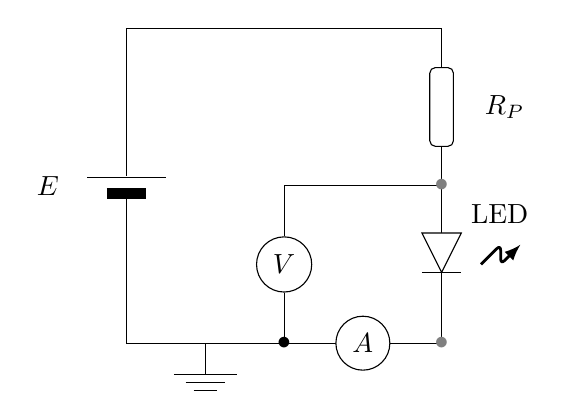
\begin{tikzpicture}
    \draw(0,-2)--(0,2)--(4,2)--(4,-2)--cycle;
    \node[fill=white, minimum height= 0.2cm] at (0,0) {}; 
    \draw(-0.5,0.1)--++(1,0);
    \draw[line width=4pt] (-0.25,-0.1)--++(0.5,0);
    
    
    %\draw[fill=white] (0,0) circle (0.5cm);
    %\draw [>=stealth, ->, very thick] (0,-0.25)--(0,0.25);
    \node at (-1,0) {$E$};
    \node[draw, fill=white, minimum width=0.3cm, minimum height=1cm, rounded corners =2pt] at (4,1) {};
    \node [xshift=0.8cm] at (4,1) {$R_{P}$};
    \draw(1,-2)--++(0,-0.4); \draw(0.6,-2.4)--++(0.8,0); \draw (0.75,-2.5)--++(0.5,0);\draw (0.85,-2.6)--++(0.3,0); 
    
    \node[circle,draw, fill =white](Voltmetre) at (2,-1) {$\operatorname{V}$};
    \draw (Voltmetre.north)|-(4,0) node[gray] {$\bullet$};
    \draw (Voltmetre.south)--(2,-2) node {$\bullet$};
    \node[circle,draw, fill =white](Ametre) at (3,-2) {$\operatorname{A}$};
    \node[gray] at (4,-2) {$\bullet$};

    %\draw (Ametre.east)--++(1,0) node (int) [midway]   {$\bullet$} --++(0,1) --++(0.4,0.8);
%\draw (0.5,2) -| (4.4,0.5);
%\draw (0.5,-1)  -|(Ametre.west);
%\draw (Voltmetre.north)--(2,2) node {$\bullet$};
%\draw (Voltmetre.south)--(2,-1) node {$\bullet$};

    
            \begin{scope}[xshift=3.75cm,yshift=-0.6cm]%LED
            \draw[fill=white] (0,0)--++(0.5,0)--++(-0.25,-0.5)--cycle;
            \draw (0,-0.5)--++(0.5,0) node[above right, yshift=0.5cm]{LED};
            \draw[->,>=latex,rounded corners=2pt, line width=1pt] (0.75,-0.4) --++ (0.25,0.25)--++(0,-0.25)--++(0.25,0.25);
            \node (A1) at (0.25,0) {};
            \node (K1) at (0.25,-0.5) {};
            \end{scope}        
\end{tikzpicture}

\end{multicols}


On fait alors varier le potentiel de la source de tension $E$, pour relever, pour plusieurs points, les valeurs du courant (A) et de la différence de potentiel (V).

La plupart des multimètres permettent d'afficher simultanément la tension et le courant continu.

Les points peuvent ensuite être enregistrés dans un fichier de tableur (type Excel ou Calc). Cet outil logiciel permettra par la suite de tracer la courbe $i=f(u)$.



\subsection*{Caractéristique Automatisée}

Une seconde méthode permettant d'\textbf{obtenir une allure de la caractéristique statique }$i=f(u)$ d'un dipôle est de faire varier la différence de potentiel à ses bornes en appliquant un signal dont l'amplitude varie lentement dans le temps. On peut alors mesurer la différence de potentiel $u$ aux bornes du dipôle et le courant $i$ le traversant à l'aide d'un oscilloscope en mode XY.

Cette méthode va nécessiter de \textbf{transformer le courant en différence de potentiel}, seule grandeur mesurable à l'aide d'un oscilloscope.

Pour faire \textbf{varier la différence de potentiel} aux bornes du dipôle, on utilisera une \textbf{générateur basse fréquence} (ou GBF).

Pour \textbf{mesurer la différence de potentiel} aux bornes du dipôle, on pourra utiliser une des voies de l'\textbf{oscilloscope} câblée en parallèle du dipôle.

Pour \textbf{mesurer le courant} traversant le dipôle, on insérera une \textbf{résistance de faible valeur} (afin de ne pas perturber le reste du montage par l'ajout d'un système de mesure) en série avec le dipôle que l'on cherche à caractériser. On pourra alors utiliser la seconde voie de l'\textbf{oscilloscope} pour mesurer la différence de potentiel aux bornes de cette résistance. Par la loi d'Ohms, on retrouvera alors la valeur du courant.

\subsubsection*{Circuit de mesure}

\begin{multicols}{2}

On donne le circuit suivant pour tracer de manière automatisée l'allure de la caractéristique statique.

\medskip


La résistance $R_P$ est une résistance de protection du dipôle à caractériser (ici une LED).

La résistance $R_I$ permet de convertir le courant traversant la branche en différence de potentiel mesurable par l'oscilloscope.

\columnbreak

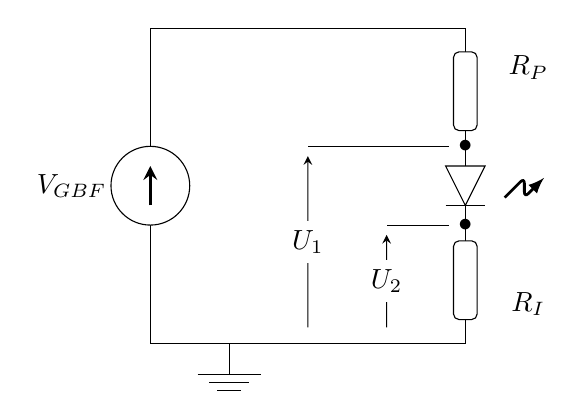
\begin{tikzpicture}
    \draw(0,-2)--(0,2)--(4,2)--(4,-2)--cycle;
    \draw[fill=white] (0,0) circle (0.5cm);
    \draw [>=stealth, ->, very thick] (0,-0.25)--(0,0.25);
    \node at (-1,0) {$V_{\text{GBF}}$};
    \node[draw, fill=white, minimum width=0.3cm, minimum height=1cm, rounded corners =2pt] at (4,1.2) {};
    \node [xshift=0.8cm] at (4,1.5) {$R_{P}$};
    \draw(1,-2)--++(0,-0.4); \draw(0.6,-2.4)--++(0.8,0); \draw (0.75,-2.5)--++(0.5,0);\draw (0.85,-2.6)--++(0.3,0); 
     \node[draw, fill=white, minimum width=0.3cm, minimum height=1cm, rounded corners =2pt] at (4,-1.2) {};
    \node [xshift=0.8cm] at (4,-1.5) {$R_I$};
            \begin{scope}[xshift=3.75cm, yshift=0.25 cm]%LED
            \draw[fill=white] (0,0)--++(0.5,0)--++(-0.25,-0.5)--cycle;
            \draw (0,-0.5)--++(0.5,0); %node[above right, yshift=0.5cm]{LED};
            \draw[->,>=latex,rounded corners=2pt, line width=1pt] (0.75,-0.4) --++ (0.25,0.25)--++(0,-0.25)--++(0.25,0.25);
            \node (A1) at (0.25,0) {};
            \node (K1) at (0.25,-0.5) {};
            \end{scope}        
            
           \node[yshift=0.25 cm]  (CH1) at (A1){$\bullet$};
            \node[yshift=-0.25 cm] (CH2)   at (K1){$\bullet$};
           \draw (CH1) --++(-2,0) node (VCH1) {};
           \draw (CH2) --++(-1,0)node (VCH2) {};
%            
           \draw [<-, >=stealth] (VCH1) -- (2,-1.8) node [midway, fill=white] {$U_{1}$};
            \draw [<-, >=stealth] (VCH2) -- (3,-1.8) node [midway, fill=white] {$U_{2}$};
\end{tikzpicture}

\end{multicols}


\subsubsection*{Méthode de mesure}

On applique un signal dont l'amplitude varie dans le temps à l'aide du GBF : un signal triangulaire par exemple à une fréquence de quelques Hertz. \textit{On s'assurera que l'amplitude du signal fourni par le GBF est inférieure aux limitations des composants du montage.}

En mesurant à l'oscilloscope les tensions $U_1$ sur une voie et $U_2$ sur l'autre voie, on accède à une image de la tension aux bornes du dipôle ($U_1 – U_2$, assimilable à $U_1$ si $U_2$ est faible pour toutes les valeurs de $i$) et à une image du courant traversant $R_I$ ($U_2$).

En traçant alors $U_2$ en fonction de $U_1$ (mode XY de l'oscilloscope), l'allure de la caractéristique statique du dipôle s'affiche alors.
\titleformat{\section}
  {\null}{}{0pt}{}

%% Docs techniques
\includepdf[pages=4, pagecommand={\section{\texorpdfstring{\hspace{-1em}}{Doc SFH206K photodiode}}}\label{doc:phdSFH206K}]{ressources/osram_SFH206K.pdf}
\includepdf[pages=5-8]{ressources/osram_SFH206K.pdf}

\includepdf[pages=3]{ressources/kingbright_LED_Rouge.pdf}
\includepdf[pages=2, pagecommand={\section{\texorpdfstring{\hspace{-1em}}{Doc Led Rouge}}}\label{doc:ledRouge}]{ressources/kingbright_LED_Rouge.pdf}
\includepdf[pages=3]{ressources/kingbright_LED_Rouge.pdf}




%% Fiches 
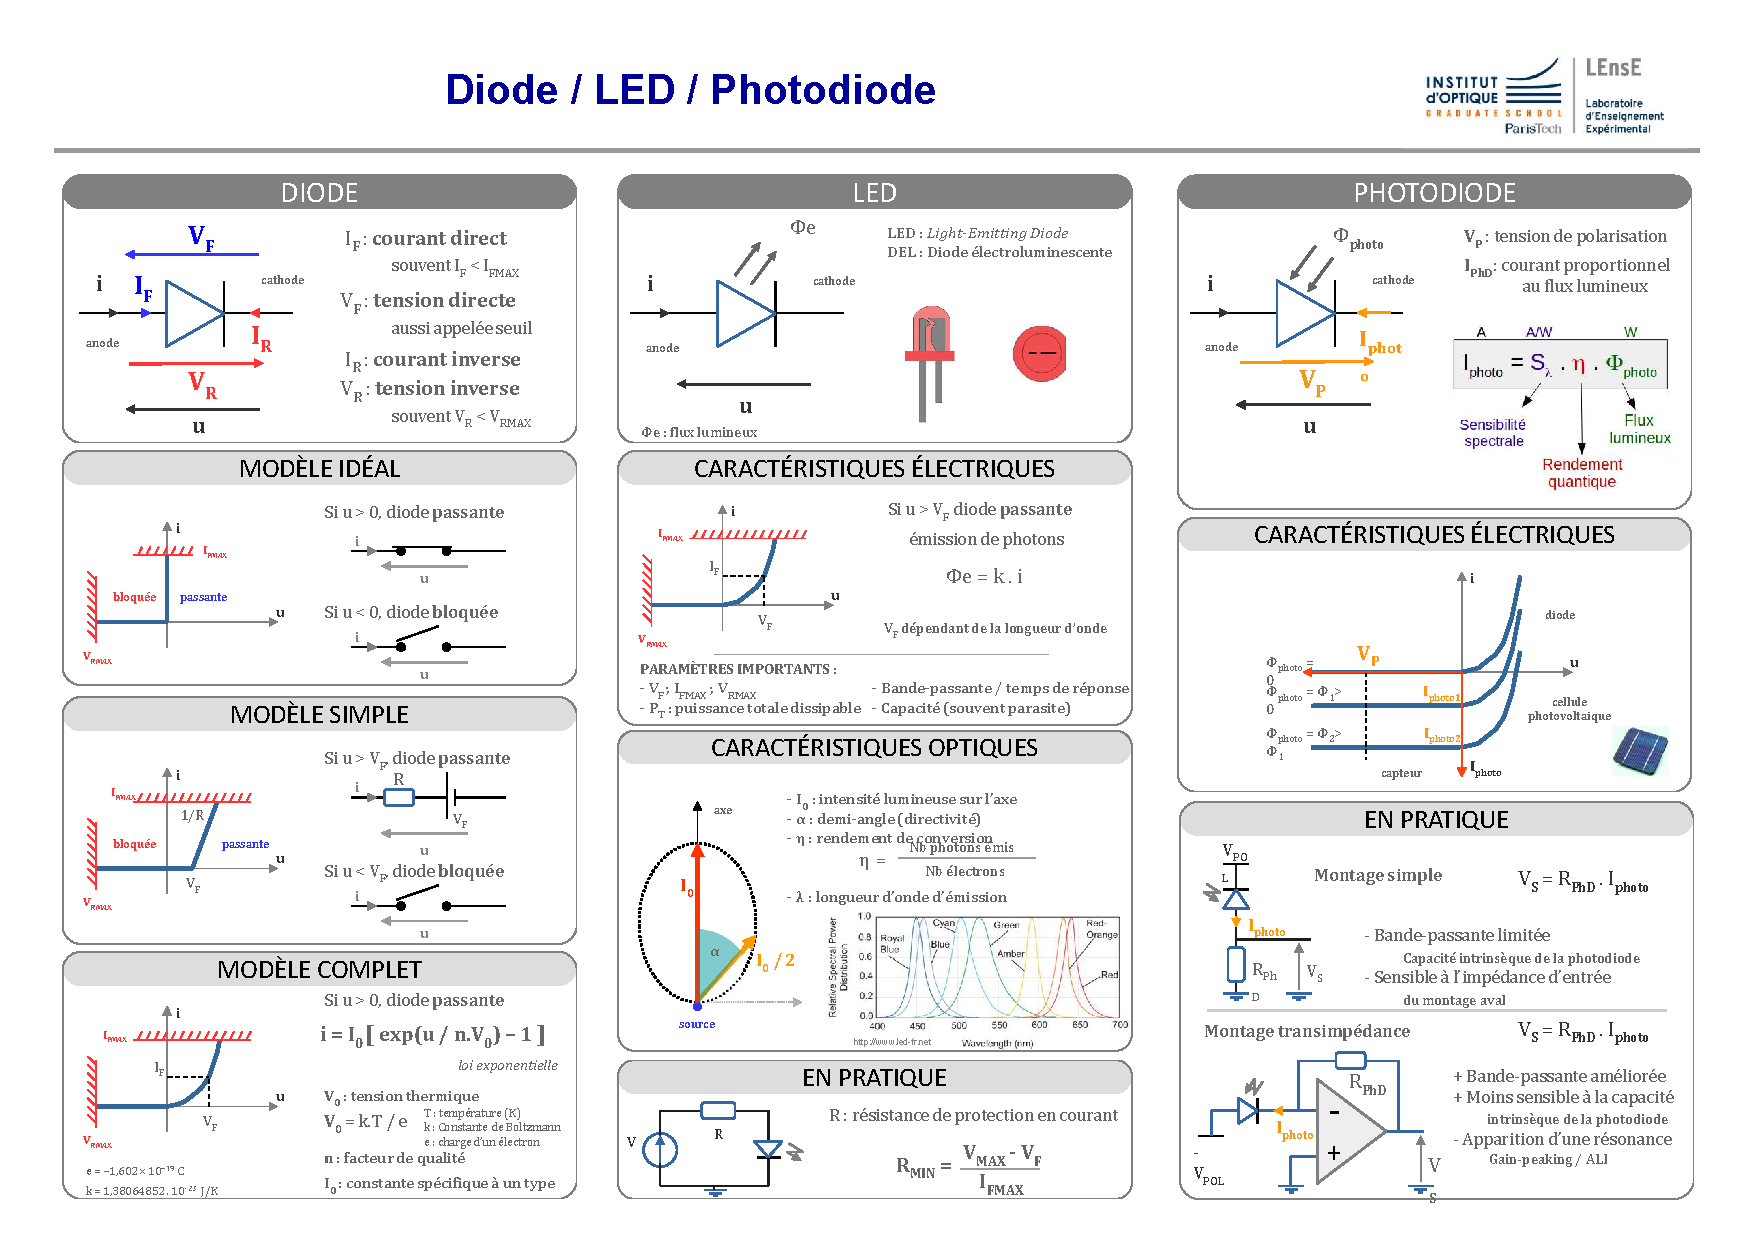
\includepdf[pages=-, landscape=true, pagecommand={\section{\texorpdfstring{\hspace{-1em}}{Fiche Diode / LED / Photodiode}}}\label{fiche:Led}]{../../Fiches/Fiche_Diode_LED_Photodiode.pdf}

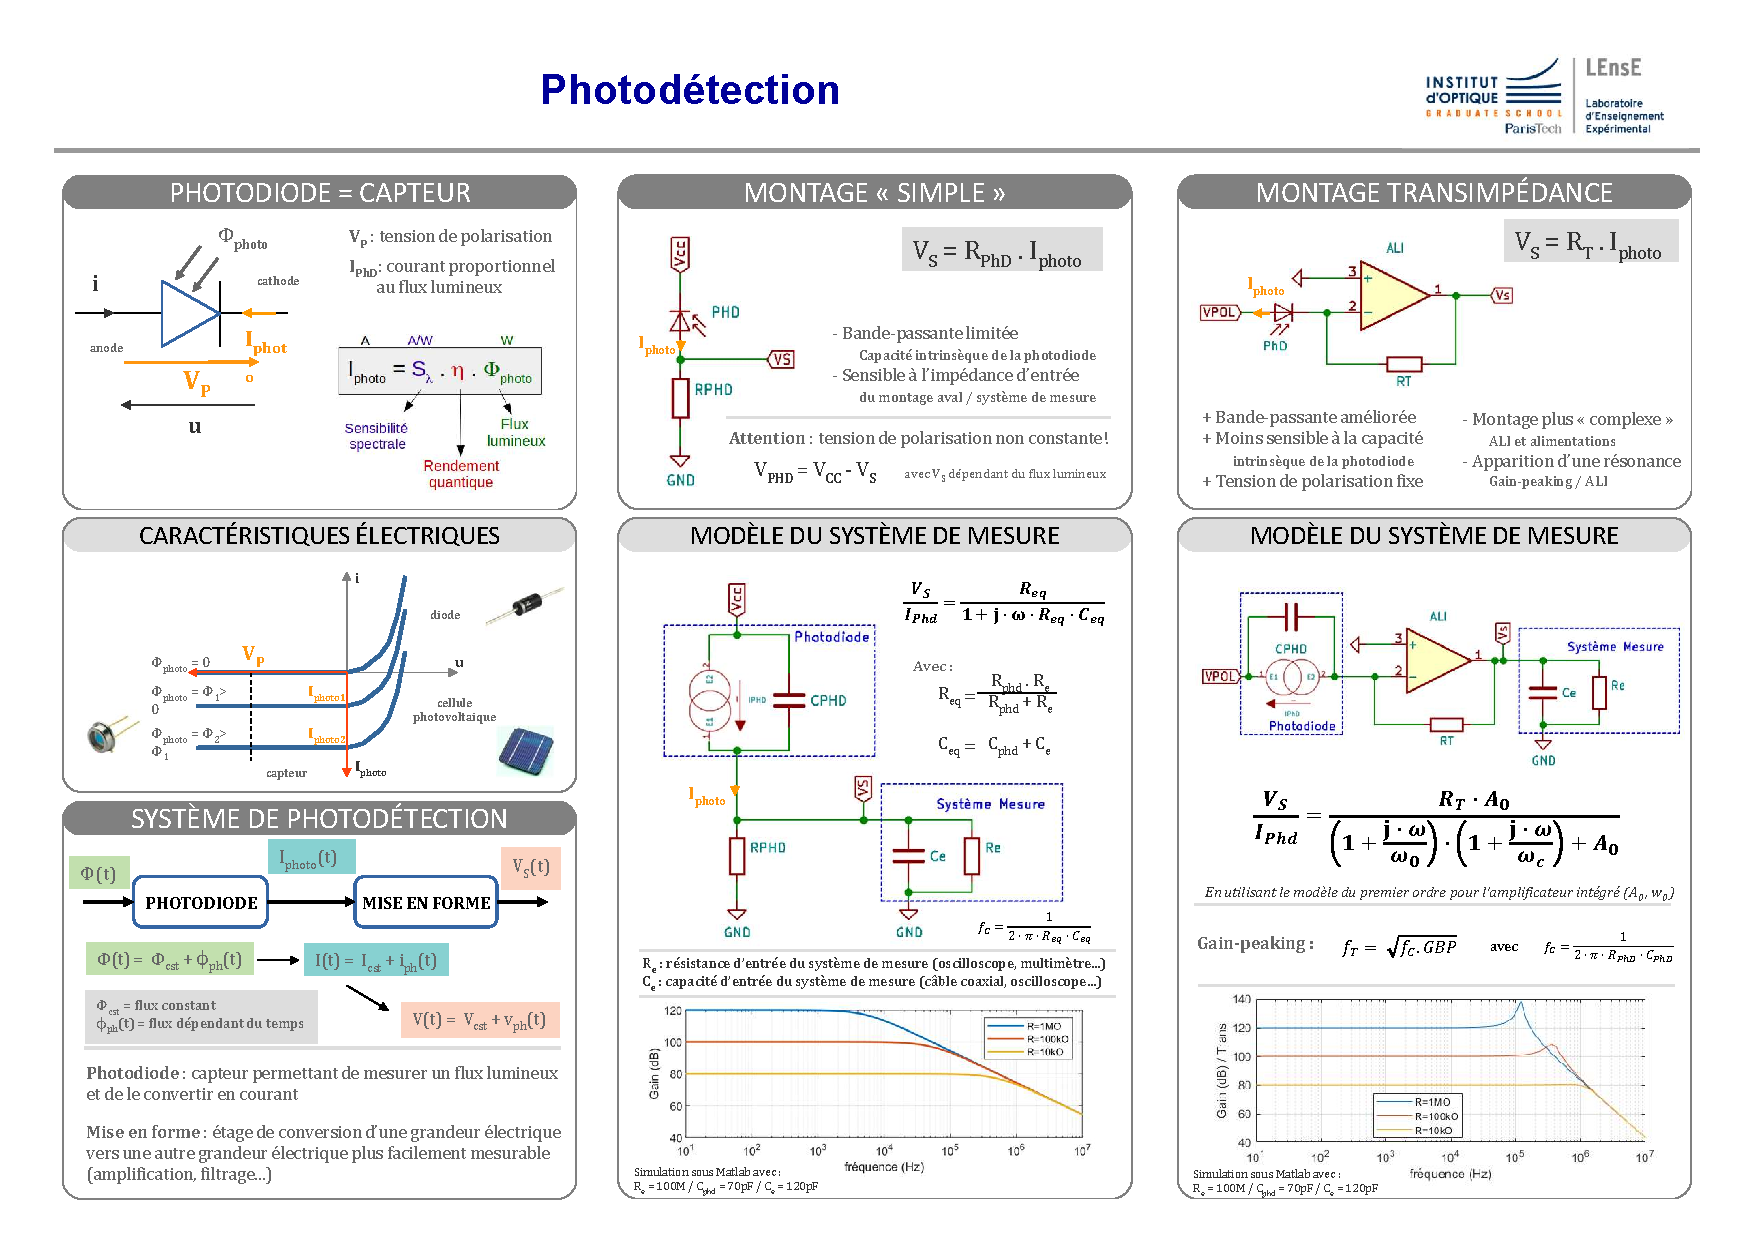
\includepdf[pages=-, landscape=true, pagecommand={\section{\texorpdfstring{\hspace{-1em}}{Fiche Photodétection}}}\label{fiche:Photodetect}]{../../Fiches/Fiche_Photodetection.pdf}



\end{document}


